\begin{figure}[h]
    \centering
    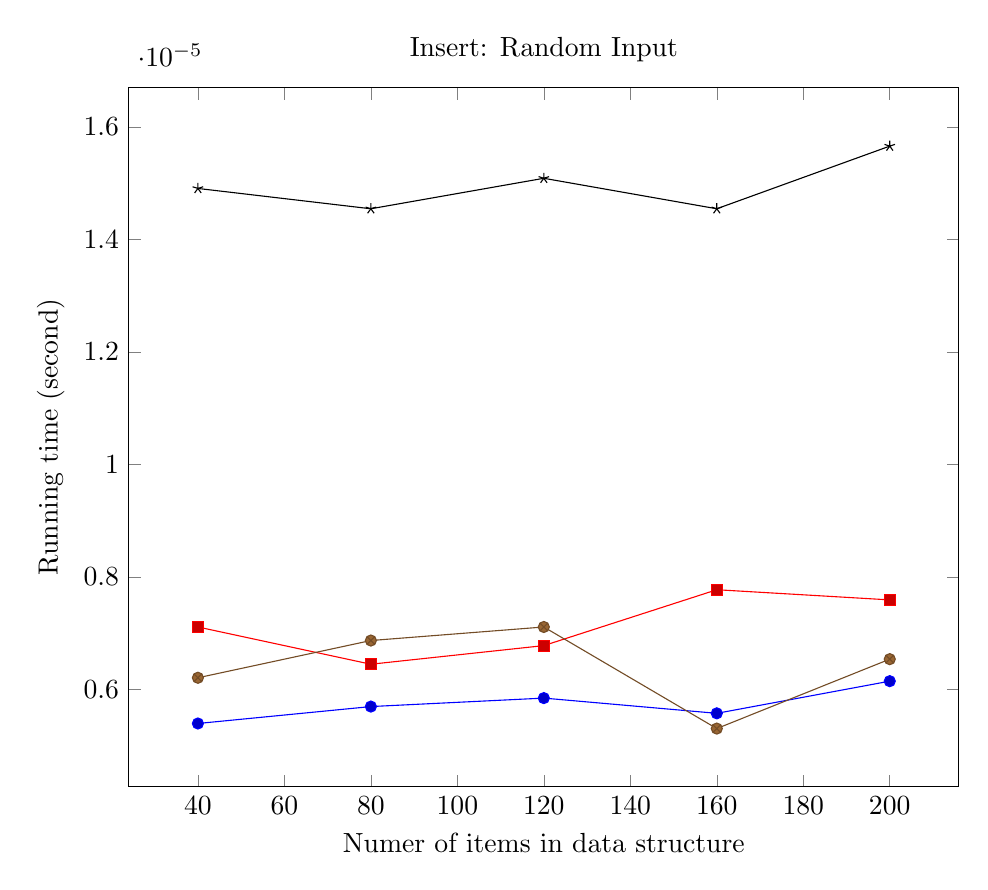
\begin{tikzpicture}
        \begin{axis}[
            xlabel={Numer of items in data structure},
            ylabel={Running time (second)},
            title={Insert: Random Input},
            width=\textwidth
        ]
		\addplot coordinates {
			(40, 5.391038527857717e-06)
			(80, 5.692213864605389e-06)
			(120, 5.842801532984776e-06)
			(160, 5.571743729909651e-06)
			(200, 6.143976869732448e-06)
		};
		\addplot coordinates {
			(40, 7.107737947342762e-06)
			(80, 6.445152206485671e-06)
			(120, 6.776445076911442e-06)
			(160, 7.770323688188752e-06)
			(200, 7.589618486142369e-06)
		};
		\addplot coordinates {
			(40, 6.2042119370830925e-06)
			(80, 6.866797677934633e-06)
			(120, 7.107737947337212e-06)
			(160, 5.300685926828974e-06)
			(200, 6.535504807508863e-06)
		};
		\addplot coordinates {
			(40, 1.490817916920406e-05)
			(80, 1.4546768765105744e-05)
			(120, 1.5088884371261546e-05)
			(160, 1.4546768765105744e-05)
			(200, 1.5661117511084344e-05)
		};
        \legend{}
        \end{axis}
    \end{tikzpicture}
    \caption{Average of 0 operations, benchmarked every 0, starting at 0.}
\end{figure}